%!TEX root = ../../thesis.tex


\section{Telluric correction}
\label{sec:telluric_correction}

\subsection{Earth's atmosphere}
\todo{move out of intro}
While the Earth's atmosphere is important for an Astronomer's lungs, it can be a nuisance for their ground-based observations.
As light form astronomical sources passes through the atmosphere, its molecular components absorb some of the light, changing spectral components observed by imprinting a transmission spectrum of our atmosphere.
The \ce{H2O} absorption is a key example as it defines the photometric and spectroscopic bands in the \nir{}. \missingfigure{example to point to}.

The correction of observations from the contamination of Earth's atmosphere is a complex process.\textbf{
    The transmission is variable on many different time scales, the water vapour change is rapid, concentrations of atmospheric constituents, to seasonal and longer.}
Such as the increase in atmospheric \ce{CO2} causing anthropamorphic climate change this requires 6\% change to \ce{CO2} line depths since 2000 Molecfit paper?
There is also variation with airmass, which depends on the observation angle in the sky and changes as targets move across the sky during the night.

other constituents, \ce{CO}, \ce{CO2}, \ce{CH4} \ldots{}, angle of observations.

An important consideration in detecting the constituents of planetary atmospheres is the characterization and removal of Earth's telluric lines.

e.g.\ 50\% error in \ce{CO2} detection on Mars atmosphere


Recently~\citet{ulmer-moll_telluric_2018} compared the telluric correction possible from three different synthetic telluric software against the standard star model.
Molecfit, a software from ESO was the most.

This is a growing field and there are other software available too\ldots{}


Water vapour content has rapid variability.
Works such as \citet{snellen_orbital_2010}, fit and remove the telluric variation during a series of observations\footnote{51 spectrum of the same target in 180 minutes for \citet{snellen_orbital_2010}}, to remove telluric lines and detect the absorption lines of exoplanet atmospheres.

\todo{finish this}


Telluric absorption map
\begin{figure}
    \centering
    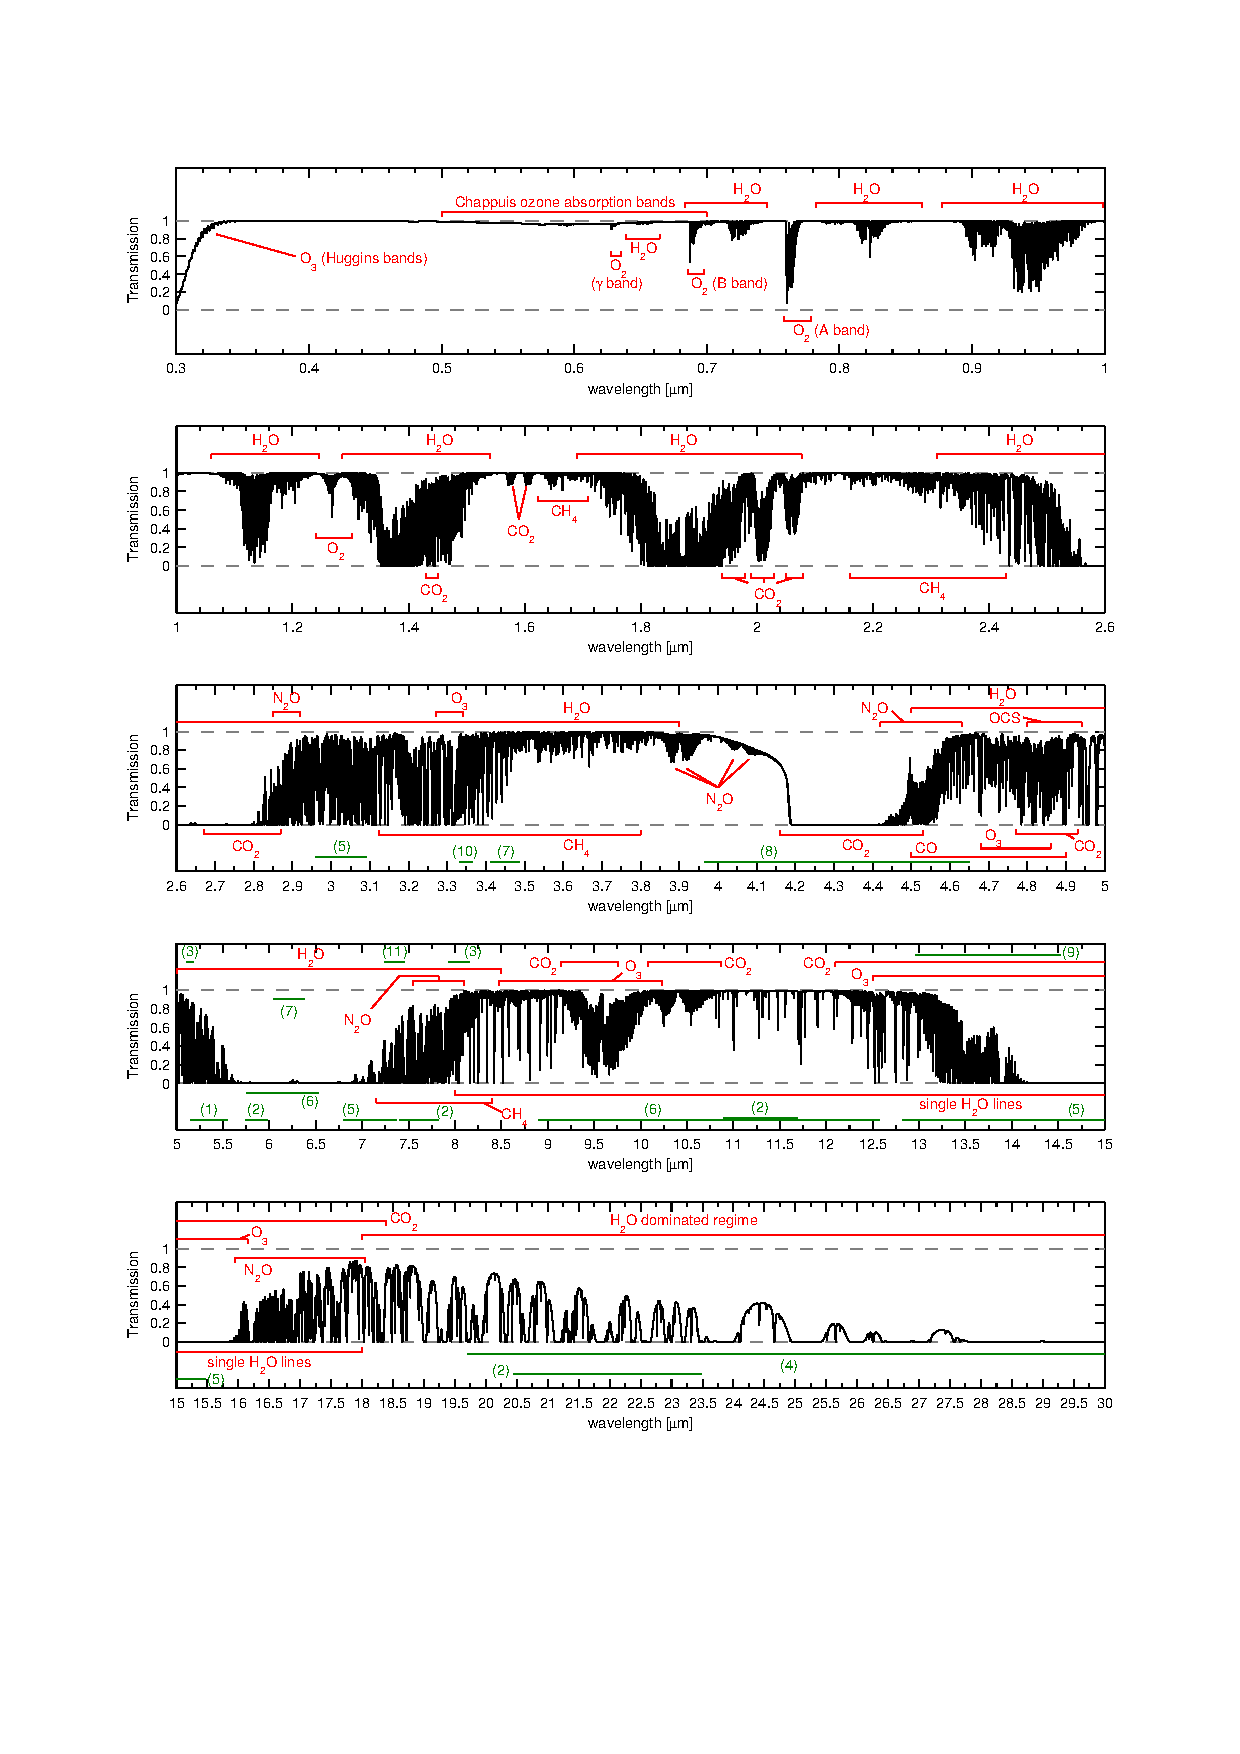
\includegraphics[width=0.9\linewidth]{figures/advanced_material/cropped_molecfit_absorbtion}
    \caption{Reproduction of Figure~1 of~\citet{smette_molecfit_2015} showing telluric absorption form 0.30 \um.
        Original caption:\textbf{add more here}}
    \label{fig:croppedmolecfitabsorbtion}
\end{figure}
\todo{Add original caption to~\cref{fig:croppedmolecfitabsorbtion}}




\subsection{Telluric models}

Utilizing telluric models has been shown to be better than the standard star method.
\subsubsection{TAPAS}
\label{subsubsec:TAPAS}

\subsection{Tapas models}
\todo{ADAPT THis section to explain the models more generally.
    Move the usage back to Reduction section}
\label{subsec:tapas_models}
For the wavelength calibration and telluric correction methods we use telluric line models.
These have been show to provide as good or better telluric correction compared to the telluric standard method \reference{telluric model correction methods original}and~\citep{ulmer-moll_telluric_2018}.

We utilized the {TAPAS} (Transmissions of the AtmosPhere for AStronomical data) web-service\footnote{\href{http://www.pole-ether.fr/tapas/}{http://www.pole-ether.fr/tapas/}}~\citep{bertaux_tapas_2014} to obtain atmospheric transmission models for each observation. {TAPAS} uses the standard line-by-line radiative transfer model code LBLRTM~\citep{clough_linebyline_1995} along with the 2008 {HITRAN} spectroscopic database~\citep{rothman_hitran_2009} and {ARLETTY} atmospheric profiles derived using meteorological measurements from the {ETHER} data center\footnote{\href{http://www.pole-ether.fr}{http://www.pole-ether.fr}} to create telluric line models.

The {ARLETTY} atmospheric profiles have a 6 hour resolution, so there may be a slight difference between the actual profile at the time of observation.

We use the mid-observation time to retrieve transmission models for each observation, with the {ARLETTY} atmospheric profiles\footnote{Nearest of the 6 hourly profiles} and vacuum wavelengths selected.
The telluric models were retrieved without any barycentric correction to keep the telluric lines at a radial velocity of zero with respect to the instrument.

{TAPAS} allows for the choice of atmospheric constituents included in the model spectra.
We obtained one model with all available species present, convolved to a resolution of \(\rm R=50\,000\), and another two models without an instrumental profile convolution applied.
For these two extra models, one contained only the transmission spectra of \ce{H2O} while the other contained all other constituents except \ce{H2O}.
This was to explore a known issue with the depth of \ce{H2O} absorption lines in the TAPAS~\citet{bertaux_tapas_2014}. \cref{subsec:telluric_correction}.


\todo{Look at} -> synthesizing telluric spectra \nir{} for {CRIRES}~\cite{seifahrt_synthesising_2010}

Using {TAPAS} is contrasted alongside Molecfit and Telfit in~\cite{ulmer-moll_telluric_2018}.
We conclude that \ldots
